%% ============================================================
%% Bachelor's Thesis — <UNIVERSITY / PROGRAM>
%% Author: Arthur Wienerroither — Student ID: h12322363
%% Adapt preamble to the official Overleaf template as needed.
%% ============================================================
\documentclass[12pt, a4paper]{report}

%% --- Encoding & language ---
\usepackage[utf8]{inputenc}
\usepackage[T1]{fontenc}
\usepackage[english]{babel}
\usepackage{csquotes}          % required by biblatex-apa

%% --- Bibliography (APA 7) ---
\usepackage[style=apa, backend=biber]{biblatex}
\addbibresource{bib.bib}

%% --- Layout ---
\usepackage[a4paper, margin=2.5cm]{geometry}
\usepackage{setspace}
\onehalfspacing

%% --- Typography ---
\usepackage[protrusion=true,expansion=false]{microtype}

%% --- Tables & figures ---
\usepackage{booktabs}
\usepackage{tabularx}
\usepackage{graphicx}
\usepackage{float}
\usepackage{longtable}
\usepackage{pdflscape}

%% --- Hyperlinks ---
\usepackage[hidelinks]{hyperref}

%% ============================================================
\begin{document}

%% --- Title page ---
\begin{titlepage}
  \centering
  \vspace*{2cm}
  {\LARGE\bfseries Organizational Conditions for AI-Driven Firm Performance\par}
  \vspace{0.5cm}
  {\large A Systematic Review of Empirical Evidence, 2015--2026\par}
  \vspace{2cm}
  {\large Bachelor's Thesis\par}
  {\large <DEGREE PROGRAM>\par}
  {\large Supervisor: PD Dr.\ Viktor Fredrich\par}
  \vspace{1cm}
  {\large Vienna University of Economics and Business (WU Wien), <TERM>\par}
  \vspace{1cm}
  {\large Arthur Wienerroither\par}
  {\large Student ID: h12322363\par}
  \vspace{0.5cm}
  {\large \today\par}
\end{titlepage}

%% --- Abstract ---
\begin{abstract}
% <Write the abstract last: context, research question, method, key findings, implications.>

\bigskip
\noindent\textbf{Keywords:} <keyword>; <keyword>; <keyword>
\end{abstract}

\newpage
\tableofcontents
\newpage

%% --- Chapters ---
\chapter{Introduction}
\label{sec:introduction}

Whether investing in artificial intelligence (AI) makes a firm more competitive is, in
Kemp's words, a theoretical puzzle \parencite[p.~618]{kemp2024competitive}\footnote{[Kemp
(2024), p.~618] ``The prospect of using artificial intelligence (AI) to establish
competitive advantages presents a theoretical puzzle.''}. The promise is large:
intelligent algorithms are expected to automate a substantial share of work and to open
new products and product-development processes. The same literature lists strategic
obstacles: AI can be myopic and hard for managers to steer, and, built on explicit
knowledge, it resembles a general-purpose
technology \parencite[p.~618]{kemp2024competitive}\footnote{[Kemp (2024), p.~618]
``Despite this promise, a growing body of research has highlighted that AI may present
substantial strategic obstacles. AI may be myopic (Balasubramanian, Ye, \& Xu, 2022),
incapable of perceiving interdependencies within a firm (Raisch \& Krakowski, 2021), and
recalcitrant to managerial control (Murray, Rhymer, \& Sirmon, 2021).'' / ``In addition,
AI is a form of explicit knowledge (Broussard, 2018; Shrestha, He, Puranam, \& von
Krogh, 2021), and resembles a general-purpose technology (Teece, 2018).''}. A
technology every competitor can buy is a poor candidate for an advantage. What firms
get out of buying it is an empirical question.

The empirical evidence has grown quickly and does not agree with itself. On German
panel data, AI use raises productivity for the yes/no measure and the intensity measure
alike \parencite[pp.~189, 201]{czarnitzki2023artificial}\footnote{[Czarnitzki et al.
(2023), p.~189] ``We analyze cross-section as well as panel data from the German part of
the European Commission's Community Innovation Survey (CIS).'' / [p.~201] ``We found
that employing AI technologies has a positive and significant impact
on firm productivity. In particular, we showed that both the use of AI and the intensity
with which firms exploit the potential of AI significantly increase both sales and
value-added.''}. Growth from AI investments concentrates among
the larger firms, and industry concentration rises
alongside \parencite[p.~1]{babina2024artificial}\footnote{[Babina et al. (2024),
p.~1] ``AI-powered growth concentrates among larger firms and is associated with higher
industry concentration.''}. Investors, on average, react to AI investment announcements
with a drop of 1.77 percent on the announcement day, and firms with weak IT bases or
poor credit ratings lose more \parencite[p.~373]{lui2022impact}\footnote{[Lui et al.
(2022), p.~373] ``The stock prices of the firms decrease by 1.77\% on the day of the
announcement. Nonmanufacturing firms and firms with weak information technology
capabilities or low credit ratings suffer a more negative impact compared with other
firms.''}. And where adoption is observed over time, it destroys old capabilities while
creating new ones at the human-machine
boundary \parencite[p.~1425]{krakowski2023artificial}\footnote{[Krakowski et al.
(2023), p.~1425] ``AI adoption triggers interrelated substitution and complementation
dynamics, which make humans' traditional competitive capabilities obsolete, while
creating new sources of persistent heterogeneity when humans interact with chess
engines.''}. Positive, negative, and conditional findings stand side by side, often for
the same outcome. The disagreement itself points at the question worth asking: under which
circumstances do the investments pay off.

That is the question this thesis asks: \emph{under what conditions do firm-level AI
investments translate into competitive advantage and superior firm performance?} The
two outcome constructs are kept analytically separate throughout, because a firm can
improve its performance without holding anything a rival cannot copy; the theoretical
grounds for that separation are laid out in Chapter~\ref{sec:background}.

The thesis answers the question with a systematic literature review of the empirical
evidence, searched over the publication window 2015 to 2026. A documented Scopus query identified 432
records, which a journal-quality filter, title-abstract screening, and full-text
screening reduced to a final corpus of 67 empirical studies; every study was coded
along a fixed scheme by two independent coders, and the resulting coding table is the
review's core deliverable. Chapter~\ref{sec:background} condenses the four theoretical
lenses used to interpret the evidence: general-purpose technologies, the resource-based
view, automation and augmentation, and situated AI. Chapter~\ref{sec:method} documents
the search, screening, and coding protocol. Chapter~\ref{sec:results} presents the
findings in two parts, a descriptive mapping of the evidence base and a synthesis of
the conditions the studies identify, ordered into six groups.
Chapter~\ref{sec:discussion} interprets the findings against the theoretical lenses and
names the limits of what the reviewed literature can show, and
Chapter~\ref{sec:conclusion} concludes.

\chapter{Theoretical Background}
\label{sec:background}

% Key concepts, definitions, and theoretical frameworks.
% Review of relevant literature; establish the state of research.

\section{Competitive advantage and firm performance}
\label{sec:constructs}

Competitive advantage is measured in 15 of the 67 studies reviewed here, and the
remaining 52 report performance outcomes only. Barney separates the two constructs by
what rivals are able to do: a firm holds a competitive advantage while it runs a
value-creating strategy no rival, actual or potential, is running at the same time, and
that advantage counts as sustained only once those rivals also cannot reproduce what the
strategy yields \parencite[p.~102]{barney1991firm}\footnote{[Barney (1991), p.~102] ``In
this article, a firm is said to have a \emph{competitive advantage} when it is
implementing a value creating strategy not simultaneously being implemented by any current
or potential competitors. A firm is said to have a \emph{sustained competitive advantage}
when it is implementing a value creating strategy not simultaneously being implemented by
any current or potential competitors \emph{and} when these other firms are unable to
duplicate the benefits of this strategy.''}. Sustained in that sense says nothing about
elapsed time. It asks whether the advantage is still there after rivals have given up
trying to copy it \parencite[p.~102]{barney1991firm}\footnote{[Barney (1991), p.~102]
``Rather, whether or not a competitive advantage is sustained depends upon the possibility
of competitive duplication. Following Lippman and Rumelt (1982) and Rumelt (1984), a
competitive advantage is sustained only if it continues to exist after efforts to
duplicate that advantage have ceased.''}. This review therefore keeps the two apart
throughout, because a firm can raise its margins without holding anything a rival is
unable to copy.

Where both constructs appear, the separation is visible in the survey items.
Chatterjee et al. ask about rivals directly: one of their competitive-advantage items
has respondents affirm that successful implementation of AI-based customer relationship
management ``will help an organization to win over its competitor which has not yet
implemented AI-CRM for B2B relationship management'' \parencite[p.~215]{chatterjee2021effect}\footnote{[Chatterjee et al. (2021),
p.~215] ``I think that successful implementation of AI-CRM will help an organization
to win over its competitor which has not yet implemented AI-CRM for B2B relationship
management.''}. Their performance items stay inside the firm and ask whether the same
system improves ``operational efficiency'' and speeds up
decisions \parencite[p.~215]{chatterjee2021effect}\footnote{[Chatterjee et al. (2021),
p.~215] ``I believe that successful implementation of AI-CRM will help the organization
to improve its operational efficiency.'' / ``I think AI-CRM helps in quick decision
making which helps the organization to improve its operational performance.''}.

Mehta et al. give competitive advantage a position between adoption and results: they
test it as the channel through which AI adoption reaches performance, and predict a
positive effect on performance in its own
right \parencite[p.~550]{mehta2025driven}\footnote{[Mehta et al. (2025), p.~550]
``H8. Competitive advantage has a significant and positive impact upon firm
performance.'' / ``H9. Competitive advantage has a mediating influence on adoption of
AI technologies and firm performance.''}.

Not every study that names competitive advantage builds its own instrument. Hossain
et al. measure sustained competitive advantage with items carried over from earlier
work \parencite[p.~247]{hossain2022marketing}\footnote{[Hossain et al. (2022), p.~247]
``sustained competitive advantage items were taken from Cao et al. (2019).''}. The
construct label alone says little about what a study measured; the items decide.

\section{Artificial intelligence as a general-purpose technology}
\label{sec:gpt}

Economists file AI under general-purpose technologies (GPTs), and that classification
already predicts an uneven payoff. A GPT earns the label because it makes ``new and
complementary production methods'' available, which can raise output over
time \parencite[p.~188]{czarnitzki2023artificial}\footnote{[Czarnitzki et al. (2023),
p.~188] ``The main feature of general-purpose technology is to enable new and
complementary production methods that may increase productivity over time (Bresnahan
and Trajtenberg 1995; Bresnahan et al., 2002; Brynjolfsson and Hitt 2003; Cardona
et al., 2013).''}. Those complements are the expensive part. Before output moves, a
firm has to redesign how work is organised, retrain staff, rework its software and
accumulate managerial experience, and because none of that accumulation is booked as
an asset, measured productivity dips before it
climbs \parencite[pp.~333--334]{brynjolfsson2021productivity}\footnote{[Brynjolfsson
et al. (2021), pp.~333--334] ``realizing their potential also requires large intangible
investments and a fundamental rethinking of the organization of production itself.
Firms must create new business processes, develop managerial experience, train workers,
patch software, and build other intangibles. This raises productivity measurement
issues because intangible investments are not readily tallied on a balance sheet or in
the national accounts.'' / [p.~334] ``The error in measured total factor productivity
growth therefore follows a J-curve shape, initially dipping while the investment rate in
unmeasured capital is larger than the investment rate in other types of capital, then
rising as growing intangible stocks begin to contribute to measured
production.''}. The lag is years, not quarters.

Two studies in this corpus show how differently that plays out at firm level. On German
innovation-survey panel data, Czarnitzki et al. measure a clear productivity gain from
AI use, for the yes/no measure and for the intensity measure
alike \parencite[pp.~189, 201]{czarnitzki2023artificial}\footnote{[Czarnitzki et al.
(2023), p.~189] ``We analyze cross-section as well as panel data from the German part of
the European Commission's Community Innovation Survey (CIS).'' / [p.~201] ``We found
that employing AI technologies has a positive and significant impact
on firm productivity. In particular, we showed that both the use of AI and the intensity
with which firms exploit the potential of AI significantly increase both sales and
value-added.''}. Fontanelli et al. ask a different question of French firms and find
that AI use raises the \emph{volatility} of productivity growth; the effect sits with
firms that buy AI from outside providers, and it weakens where more of the payroll is
made up of ICT engineers and
technicians \parencite[pp.~1--2]{fontanelli2025predictive}\footnote{[Fontanelli et al.
(2025), p.~1] ``This paper shifts the focus and investigates the impact of predictive AI
on the volatility of firms' productivity growth rates.'' / ``Using firm-level data from
the 2019 French ICT survey, we provide robust evidence that AI use is associated with
increased volatility.'' / [pp.~1--2] ``Our results show that heightened volatility is concentrated among AI
buyers, whereas firms that develop AI internally experience no such association.
Finally, we find that the AI-volatility link among `AI buyers' is mitigated in firms
with a higher share of ICT engineers and technicians, suggesting that AI's successful
integration requires complementary human capital.''}. Across the two results, the
reading this review takes forward is that the same AI investment can stand behind
either outcome; what differs between the firms is the complements.

\section{The resource-based view and the imitability problem}
\label{sec:rbv}

Across the studies reviewed here, the resource-based view (RBV) is the recurring reason
given for expecting AI to pay off. Barney sets four conditions on a resource before it
can hold an advantage in place: it has to be valuable, rare among competitors and
imperfectly imitable, and no substitute may do the same strategic
job \parencite[pp.~105--106]{barney1991firm}\footnote{[Barney (1991), pp.~105--106] ``To
have this potential, a firm resource must have four attributes: (a) it must be valuable,
in the sense that it exploit opportunities and/or neutralizes threats in a firm's
environment, (b) it must be rare among a firm's current and potential competition, (c) it
must be imperfectly imitable, and (d) there cannot be strategically equivalent substitutes
for this resource that are valuable but neither rare or imperfectly imitable.''
Typographical errors as in the original.}. Alwakid and Dahri restate the four conditions
as the VRIN
acronym \parencite[p.~14]{alwakid2025harnessing}\footnote{[Alwakid \& Dahri (2025), p.~14]
``Traditionally, RBV posits that firms achieve sustained competitive advantage by
strategically deploying valuable, rare, inimitable, and non-substitutable (VRIN)
resources (Barney, 1991; Wang \& Zhang, 2025).''}. That is a shorthand Barney himself comes close
to when he lists ``rareness, inimitability, non-substitutability'' among the
characteristics that can qualify a firm attribute as a source of advantage, adding that
the attribute becomes a resource only once it exploits an opportunity or neutralizes a
threat \parencite[p.~106]{barney1991firm}\footnote{[Barney (1991), p.~106] ``Firm
attributes may have the other characteristics that could qualify them as sources of
competitive advantage (e.g., rareness, inimitability, non-substitutability), but these
attributes only become resources when they exploit opportunities or neutralize threats in
a firm's environment.''}. Hossain et al. put the same argument
in terms of what a firm does with what it owns, and tie the long-run case to holdings
rivals cannot match \parencite[pp.~241--242]{hossain2022marketing}\footnote{[Hossain
et al. (2022), pp.~241--242] ``The resource-based view (RBV) portrays how a firm can
optimally use its resources, which are non-substitutable, unique and valuable for
achieving sustained competitive advantage (Wernerfelt, 1984).''}.

Purchased AI fails that test, and the RBV literature says so plainly. Krakowski et al.
note that AI costs almost nothing to reproduce and that little stands in the way of
copying it, so where AI substitutes a human capability, the RBV predicts that the
advantage resting on that capability will
erode \parencite[p.~1426]{krakowski2023artificial}\footnote{[Krakowski et al.
(2023), p.~1426] ``When AI substitutes humans' cognitive capabilities, the RBV expects
the advantage that these capabilities provided to erode (Peteraf \& Bergen, 2003). This
is because, as a technology resource, AI has close to zero marginal reproduction costs
and few imitation barriers (Brynjolfsson \& McAfee, 2014, p.~31).''}. Their own evidence
relocates the advantage rather than denying it: what resists imitation is the combination
a firm builds, not either side of
it \parencite[p.~1446]{krakowski2023artificial}\footnote{[Krakowski et al. (2023),
p.~1446] ``Our findings show that humans remain sources of sustainable advantage by
combining and integrating their capabilities with machine capabilities into uniquely
complementary bundles (Argyres \& Zenger, 2012).'' / ``the locus of sustainable advantage
is neither human nor machine capabilities, but what humans do with these capabilities.''}.

Two consequences follow for this review. The RBV speaks to competitive advantage and not
to performance, so a study reporting higher margins has not thereby shown that anything
is defensible against rivals; the separation of the two constructs in
Section~\ref{sec:constructs} is a theoretical requirement, not only a coding convention.
And if the resource itself is imitable, the variation worth studying lies in what
surrounds it, which is why the conditions under which AI pays off are treated here as the
object of analysis rather than as controls.
% Barney (1991) wird ueber literature/barney1991firm.txt zitiert (verifiziertes
% Text-Sidecar zum Bildscan, Seitenmarker = Journalseiten). Alle Passagen am
% Seitenbild gegengelesen: S. 102 (Definitionen, in Abschnitt 2.1) sowie
% S. 105-106 und S. 106 (vier Attribute, hier).

\section{Automation and augmentation}
\label{sec:autoaug}

The same investment can be deployed in two ways, and the strategy literature keeps them
apart. Raisch and Krakowski define automation as machines taking a task over from a
human, and augmentation as humans and machines working on a task
together \parencite[p.~192]{raisch2021artificial}\footnote{[Raisch \& Krakowski (2021),
p.~192] ``Whereas automation implies that machines take over a human task, augmentation
means that humans collaborate closely with machines to perform a task.''}. Their argument
against the popular advice to prefer augmentation is that the two cannot be held apart in
practice. For any single task at any single moment the firm picks one approach, and that
choice makes the two contradictory; widen the frame to several tasks over several years
and each turns out to produce the other, which makes them
interdependent \parencite[pp.~195--197]{raisch2021artificial}\footnote{[Raisch \&
Krakowski (2021), p.~195] ``Automation and augmentation are contradictory, because
organizations choose either one or the other approach to address a given task at a
specific point in time.'' / ``If we increase our analysis's temporal scale (from one
point in time to its evolution over time) and spatial scale (from one to multiple
tasks), we comprehend that, in the management domain, the two AI applications are not
only contradictory but also interdependent.'' / [p.~196] ``Consequently, augmentation
may enable a transition to automation over time.'' / [p.~197] ``Automation in one task
`spills over,' enabling adjacent tasks' augmentation.''}.

Corpus studies pick the distinction up as a design choice with different returns. Zebec
and Indihar {\v S}temberger treat the two as the use cases through which AI adoption
reaches performance, automation paying off in efficiency and augmentation in what people
and machines manage
jointly \parencite[p.~7]{zebec2024creating}\footnote{[Zebec \& Indihar {\v S}temberger
(2024), p.~7] ``Automation involves machines taking over tasks from humans, leading to
performance gains via resource, cost and information-processing efficiencies. In
contrast, augmentation involves humans collaborating with machines, enhancing both human
and machine skills and productivity.''}. Their model then returns no significant direct
effect of process automation on process performance once tasks become complex, and the
recommendation they draw from it is a boundary condition: automate what is routine,
augment what is
ambiguous \parencite[pp.~16--17]{zebec2024creating}\footnote{[Zebec \& Indihar
{\v S}temberger (2024), pp.~16--17] ``The results show that BPA has no significant direct
effect on BPP for more complex tasks in terms of efficiency of execution or scalability.''
/ ``In summary, automate routine, well-structured tasks and augment complex, ambiguous
ones.''}. Where the line falls is itself unstable. In the fragrance industry the machine
took over part of the perfumers' problem solving and could not touch the part that
depends on smelling a scent and judging how people will react to
it \parencite[p.~1445]{krakowski2023artificial}\footnote{[Krakowski et al. (2023),
p.~1445] ``While machines substitute perfumers regarding certain problem solving
activities, they are unable to match the perfumers' unique ability to smell fragrances
and predict the human emotions they trigger. This example illustrates that AI is likely
to substitute some, but not all of complex business tasks' activities.''}.

\section{Situated AI}
\label{sec:situated}

Kemp starts from the puzzle the two previous sections produce: AI is available to
everyone, so buying it should not yield an advantage, yet firms plainly differ in what
they get out of it. His answer is situated AI, which he defines as AI hemmed in by the
firm's own experience, structure and
relationships \parencite[p.~618]{kemp2024competitive}\footnote{[Kemp (2024), p.~618]
``The present paper begins to resolve this puzzle by developing a theory of situated
AI---AI whose agency is circumscribed in a firm's experiential, structural, and
relational systems.''}. Three properties of the technology stand in the way, and the
first of them is the imitability problem from Section~\ref{sec:rbv} under another name:
AI is generic, explicit and myopic. Being generic puts AI on a level with general human
capital, which competitors can acquire and put to work much as the adopter
does \parencite[p.~620]{kemp2024competitive}\footnote{[Kemp (2024), p.~620] ``The generic,
explicit, and myopic nature of AI all endanger its firm-level benefits, but are uniquely
difficult to surmount because AI is both a machine and agentic (Smith \& Lewis, 2011).
For example, AI's generic nature is akin to general human capital. General human capital
cannot typically underly interfirm advantages because a firm's competitors can usually
acquire and deploy that knowledge in ways that closely mimic corresponding actions of the
focal firm.''}.

What a firm does control is the situating. Kemp names three activities: grounding, which
picks the experiences a firm's own AI learns from; bounding, which works on the
experiences feeding a competitor's AI; and recasting, which keeps reworking the
algorithms and the routines around them so the AI stays aligned with the rest of the
firm's activities \parencite[pp.~618--619]{kemp2024competitive}\footnote{[Kemp (2024),
pp.~618--619] ``Grounding involves orchestrating which experiences one's AI will be
allowed to learn from across the organization. Bounding involves efforts to shape the
experiences anchoring a competitor's AI. Recasting involves orchestrating the continual
adaptation of algorithms and their surrounding routines to enhance AI's alignment with
interdependent activities in a firm.''}. The vocabulary is conditional throughout. None
of the three is a property of the technology, and each is something a firm may or may not
do.

Empirical work in the corpus starts from the same reading. Shi et al. take the mixed
results of earlier work as a sign that what AI yields depends on intangible complements,
on governance, and on managerial capability bound to its context, and they test that
claim on Chinese listed firms, with data assets as the channel and managerial capability
as the moderator \parencite[p.~1]{shi2025value}\footnote{[Shi et al. (2025), p.~1] ``Drawing on a
comprehensive dataset of Chinese listed companies spanning 2010--2022, this study
investigates how AI adoption influences enterprise value through the mediating role of
data assets and the moderating effect of managerial capability.'' / ``These mixed
outcomes suggest that the value-creating capacity of AI depends on more than technological
sophistication alone; it hinges on complementary intangible resources, effective
governance structures, and context-specific managerial capabilities---factors that current
empirical research has only partially explored.''}. Kemp's paper is conceptual, so what it
offers are propositions rather than findings. They are the propositions this review is
positioned to examine, because the conditions Kemp derives are the conditions the coded
studies report.

\chapter{Method}
\label{sec:method}

% Research design and approach.
% Data collection / literature search strategy, databases, inclusion criteria.
% Analysis procedure.

% TODO beim Ausschreiben dieses Kapitels uebernehmen (Transparenzhinweis zur
% Zitierweise, Regel eingefroren 28.07.2026, Begruendung in CLAUDE.md):
%
% Seven of the 67 studies carry no printed page numbers. Three of them appear in
% Elsevier journals that number articles instead of pages, and are cited by their
% article number with the article-internal page \parencite[e.g.][p.~5]{babina2024artificial}.
% The remaining four are paginated relative to the article by their publisher or had
% not been assigned to an issue at the time of retrieval, and are cited by section
% \parencite[e.g.][sec.~5.1]{banna2025value}. No PDF page is reported as a printed
% journal page anywhere in this thesis.

\chapter{Results}
\label{sec:results}

% Part 1: descriptive mapping (this file, drafted 18 July 2026).
% Part 2: analytical synthesis of conditions — next writing step.
% All numbers below are derived from corpus/coding_table.csv (n = 67, all rows final);
% figures generated by corpus/make_figures.py.

This chapter reports the evidence in two steps. Section~\ref{sec:results-mapping} maps the 67 included studies descriptively: where the evidence comes from and how it is produced. Section~\ref{sec:results-synthesis} then synthesizes the conditions under which firm-level AI investments translate into performance gains or competitive advantage. All counts, groupings, and figures in this chapter are the author's own compilation from the coding table; the full table is reported in the appendix.

\section{Descriptive mapping of the evidence base}
\label{sec:results-mapping}

The search window ran from 2015 to 2026, yet the earliest included study dates from 2020 (Figure~\ref{fig:year}). Growth is concentrated at the end of that window: 44 of the 67 studies, two thirds of the corpus, appeared in 2025 and 2026 alone. The evidence base is young.

\begin{figure}[htbp]
  \centering
  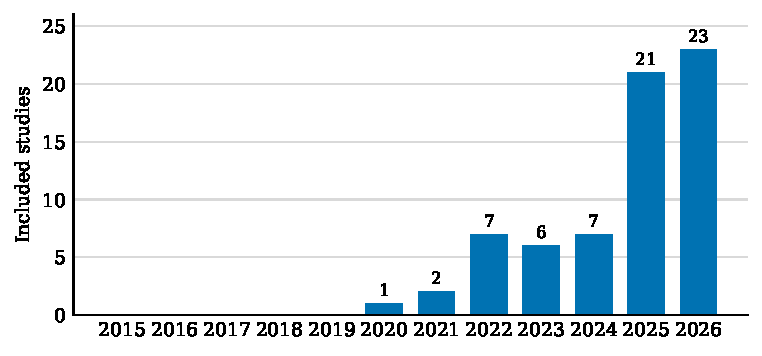
\includegraphics[width=\textwidth]{figures/fig_year}
  \caption{Included studies per publication year, search window 2015--2026 (n = 67). Source: own representation based on the coding table.}
  \label{fig:year}
\end{figure}

The 67 studies are spread across 45 journals, with no dominant outlet: Industrial Marketing Management and the Journal of Business Research lead with five studies each, followed by Technology in Society, the International Review of Financial Analysis, and the International Journal of Information Management with four each. Journal quality within the corpus is skewed toward the middle of the AJG scale (Figure~\ref{fig:ajg}): 27 studies come from journals rated 2, another 33 from journals rated 3, and seven from journals rated 4 or 4*.

\begin{figure}[htbp]
  \centering
  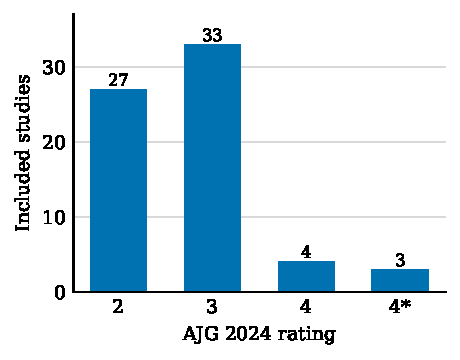
\includegraphics[width=0.55\textwidth]{figures/fig_ajg}
  \caption{Included studies by AJG 2024 journal rating (n = 67). Source: own representation based on the coding table.}
  \label{fig:ajg}
\end{figure}

Two research designs dominate the corpus (Figure~\ref{fig:method}): panel econometrics on archival firm data (27 studies) and survey-based structural equation modeling (24 studies). The remaining sixteen studies combine several methods (six), examine stock market reactions in event studies (four), or build on case evidence (three); fsQCA, data envelopment analysis, and survey-based regression appear once each. The way studies operationalize AI investment splits the corpus in half: 33 studies rely on managers' self-reports through survey constructs, 31 on archival measures, and three on qualitative observation. Disclosure text mining (seven studies), patent-based proxies (six), workforce-based measures such as AI job postings (five), and investment announcements (four) account for most of the archival measures; the remaining nine rest on single-study instruments, for example procurement records or exposure to an AI policy shock.

\begin{figure}[htbp]
  \centering
  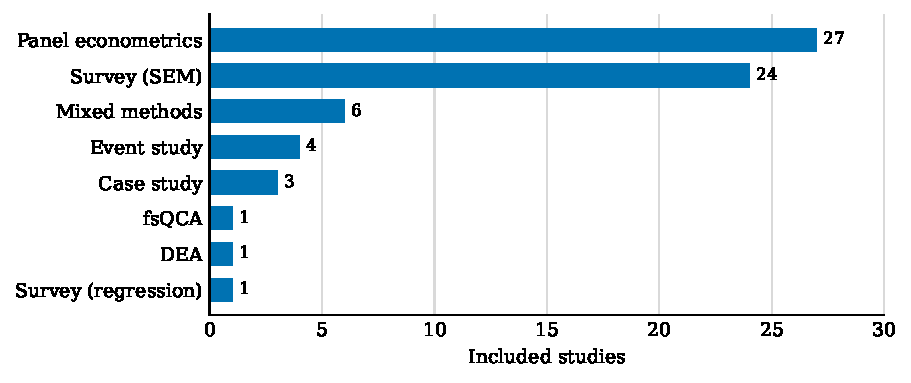
\includegraphics[width=\textwidth]{figures/fig_method}
  \caption{Included studies by research design (n = 67). Source: own representation based on the coding table.}
  \label{fig:method}
\end{figure}

Study samples cluster in two countries (Figure~\ref{fig:geography}): the USA and China account for 16 studies each, together almost half of the corpus. India follows with seven studies, and another seven draw on multi-country samples. European firms appear in ten studies: four multi-country European samples plus six single-country ones. Most samples span several industries: 39 studies are cross-industry, ten focus on manufacturing, and the rest examine single settings such as healthcare or high-tech ventures.

\begin{figure}[htbp]
  \centering
  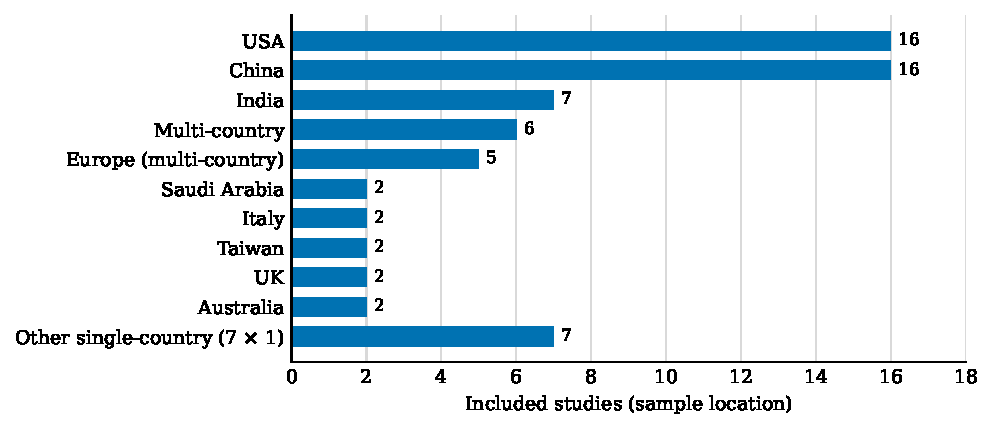
\includegraphics[width=\textwidth]{figures/fig_geography}
  \caption{Included studies by sample location (n = 67). Source: own representation based on the coding table.}
  \label{fig:geography}
\end{figure}

Following the distinction between superior firm performance and competitive advantage introduced in Chapter~\ref{sec:background}, the coding recorded which of the two constructs each study measures (Figure~\ref{fig:outcome}). The result is one-sided: 52 of the 67 studies measure firm performance only. Six measure competitive advantage as a distinct construct, and nine measure both. Measured competitive advantage is thus rare in this literature: 15 studies, under a quarter of the corpus. Effect directions spread across all four codes: 38 studies report a positive average effect of AI investment on their outcome, 20 an effect that exists only through a mechanism or under specific circumstances, five results that split across outcome indicators, and four negative effects. Among the 15 studies with a competitive-advantage construct, ten find positive and five conditional effects; none reports a negative one.

\begin{figure}[htbp]
  \centering
  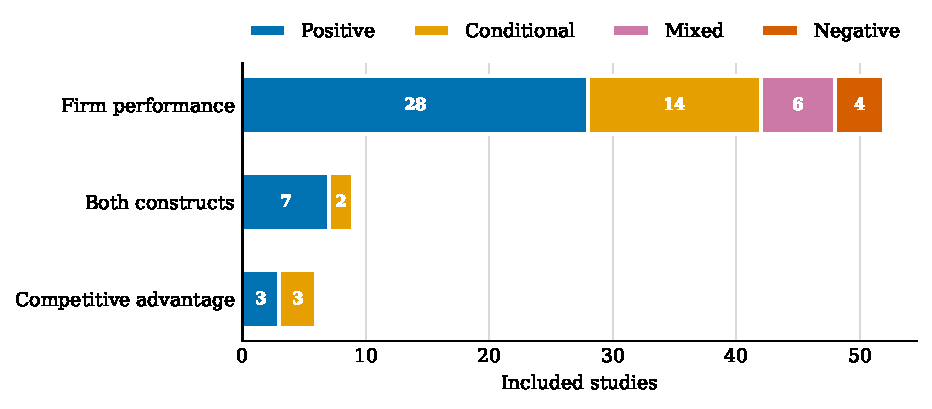
\includegraphics[width=\textwidth]{figures/fig_outcome_direction}
  \caption{Outcome construct by reported effect direction (n = 67). Source: own representation based on the coding table.}
  \label{fig:outcome}
\end{figure}

Conditions are the rule, not the exception: 63 of the 67 studies identify at least one moderator, mediator, complement, or threshold that shapes the link between AI investment and its outcome. Only four studies report unconditional evidence. Section~\ref{sec:results-synthesis} orders these conditions.

\section{Synthesis of conditions}
\label{sec:results-synthesis}

% Part 2 — analytical synthesis of the identified conditions (next writing step).

\chapter{Discussion}
\label{sec:discussion}

% Restate the research question. Interpret the results.
% Situate findings in the current debate; point at open questions.

\chapter{Conclusion}
\label{sec:conclusion}

This thesis asked under what conditions firm-level AI investments translate into
competitive advantage and superior firm performance, and answered it with a systematic
review of 67 empirical studies published between 2020 and 2026, drawn from a documented
Scopus search of 432 records, screened in three recorded stages, and coded by two
independent coders against a frozen scheme. The coding table in the appendix is the
review's core deliverable; every number in the text derives from it.

The answer favors conditions over the investment itself. Across the corpus, 38 of the
67 studies report positive average effects, and the evidence is conditional almost
throughout: 63 studies identify at least one condition
that decides whether the investment reaches its outcome. The review ordered these
conditions into six groups, from the complementary investments a firm makes alongside
the technology to the credibility with which the investment is communicated. For
competitive advantage, the evidence is thin. 15 studies measure the construct, almost
always as a perceived edge at one point in time, and only a single study in the corpus
follows an advantage against imitation over time.

The contribution is the ordered map itself. Where individual studies report single
moderators and mediators, the review shows that the conditions recur in patterned
groups across methods and settings, that the configurational evidence finds them
working in combination rather than alone, and that the two outcome constructs the field
often blends carry different amounts of evidence. The map marks where the next studies
are needed, with persistence the least covered and most consequential claim. Firms can
read the same map as a checklist of what has to be in place before the investment can
be expected to pay.


%% --- References ---
\newpage
\printbibliography[heading=bibintoc, title={References}]

%% --- Appendix ---
\newpage
\appendix
\chapter*{Appendix}
\addcontentsline{toc}{chapter}{Appendix}

\section*{Coding table}
\label{app:coding}

\noindent The full coding table for all 67 included studies, split into study characteristics (Table~\ref{tab:coding-a1}) and findings (Table~\ref{tab:coding-a2}).
% Generated by corpus/make_appendix_table.py from corpus/coding_table.csv — regenerate, never hand-edit.

% AUTO-GENERATED by corpus/make_appendix_table.py — do not edit by hand.
\begingroup
\renewcommand{\thetable}{A.\arabic{table}}
\setcounter{table}{0}
\begin{landscape}
\scriptsize
\begin{longtable}{@{}l p{2.6cm} p{3.4cm} p{1.8cm} p{5.0cm} p{2.1cm} p{6.2cm}@{}}
\caption{Included studies: characteristics and design (n = 67). Source: author's compilation.}\label{tab:coding-a1}\\
\toprule
ID & Study & Journal (AJG) & Country & Sample & Method & AI investment measure \\
\midrule
\endfirsthead
\multicolumn{7}{@{}l}{\tablename~\thetable{} (continued)}\\
\toprule
ID & Study & Journal (AJG) & Country & Sample & Method & AI investment measure \\
\midrule
\endhead
\bottomrule
\endfoot
S01 & Wamba-Taguimdje et al. (2020) & Business Process Management Journal (2) & multi-country & \textasciitilde{}500 vendor-published AI project cases & case study & case observation (vendor project reports) \\
\addlinespace[2pt]
S02 & Baabdullah et al. (2021) & Industrial Marketing Management (3) & Saudi Arabia & 392 B2B SMEs & survey-SEM & survey construct (acceptance of AI practices) \\
\addlinespace[2pt]
S03 & Chatterjee et al. (2021) & Industrial Marketing Management (3) & India & 349 managers & survey-SEM & survey construct (AI-CRM implementation) \\
\addlinespace[2pt]
S04 & Chatterjee et al. (2022) & Journal of Business Research (3) & India & 312 manager responses & survey-SEM & survey construct (AI-embedded CRM adoption) \\
\addlinespace[2pt]
S05 & Hossain et al. (2022) & Industrial Marketing Management (3) & Bangladesh & 257 manager responses & survey-SEM & survey construct (AI adoption on a marketing analytics platform) \\
\addlinespace[2pt]
S06 & Lee et al. (2022) & Technovation (3) & South Korea & 160 high-tech firms & panel econometrics & survey (AI-adoption intensity) linked to financial records \\
\addlinespace[2pt]
S07 & Leoni et al. (2022) & International Journal of Operations and Production Management (4) & Italy & 120 senior executives & survey-SEM & survey construct (AI adoption/use) \\
\addlinespace[2pt]
S08 & Lui et al. (2022) & Annals of Operations Research (3) & USA & 119 AI investment announcements by 62 listed firms, 2015-2019 & event study & announcements (AI investment announcements) \\
\addlinespace[2pt]
S09 & Mishra et al. (2022) & Journal of the Academy of Marketing Science (4*) & USA & 19,000 firm-year observations of US-listed firms & panel econometrics & annual-report text (share of AI-related keywords) \\
\addlinespace[2pt]
S10 & Sun et al. (2022) & Systems Research and Behavioral Science (2) & China & 234 AI-related manufacturers (general-manager/CEO respondents) & survey-SEM & survey construct (value co-creation in AI innovation ecosystem) \\
\addlinespace[2pt]
S11 & Ali et al. (2023) & Journal of Organizational Change Management (2) & UAE & single hospital case (Dubai): 9 interviews with the robotic-surgery team plus archival data & case study & case observation (adoption of AI/robotic surgery) \\
\addlinespace[2pt]
S12 & Czarnitzki et al. (2023) & Journal of Economic Behavior and Organization (3) & Germany & 5,851 firms (409 AI users), representative German innovation survey 2018 & panel econometrics & survey (AI adoption yes/no plus intensity of AI use in business processes) \\
\addlinespace[2pt]
S13 & Huang \& Lee (2023) & Data Base for Advances in Information Systems (2) & USA & 109 AI implementation announcements by S\&P 500 firms, 2014-2019 & event study & announcements (AI implementation) \\
\addlinespace[2pt]
S14 & Krakowski et al. (2023) & Strategic Management Journal (4*) & multi-country & same chess players across human-only, human-plus-AI and engine-only tournaments (controlled competitive setting) & panel econometrics & adoption of chess engines (AI) in competitive play \\
\addlinespace[2pt]
S15 & Samadhiya et al. (2023) & Industrial Marketing Management (3) & India & interviews with senior B2B managers plus a survey of 142 responses & mixed & survey construct (AIPRM capabilities: AI-based partner relationship management) \\
\addlinespace[2pt]
S16 & Wu \& Monfort (2023) & Psychology and Marketing (3) & Taiwan & 278 CEO/marketing-manager responses, food franchises and chain stores, 2020 & survey-SEM & survey construct (implementation of AI marketing strategy) \\
\addlinespace[2pt]
S17 & Babina et al. (2024) & Journal of Financial Economics (4*) & USA & 1,993 US listed firms & panel econometrics & resume-based (share of AI-skilled workers as a proxy for firm AI investment) \\
\addlinespace[2pt]
S18 & Cannas et al. (2024) & International Journal of Production Research (3) & Italy & 6 companies, 17 AI implementation cases, interview-based & case study & case observation (AI applications across supply-chain processes) \\
\addlinespace[2pt]
S19 & Pesqueira et al. (2024) & Computers and Industrial Engineering (2) & Europe & 4 pharmaceutical companies (2 AI adopters vs. 2 non-adopters) plus a two-round expert panel of 53 & mixed & adoption status (AI in tender management) \\
\addlinespace[2pt]
S20 & Pham et al. (2024) & Journal of Business Research (3) & USA & 941 AI and 941 matched non-AI hospital-year observations (246 hospitals), US, 2000-2020 & panel econometrics & adoption dummy (hospital has adopted AI or not) \\
\addlinespace[2pt]
S21 & Sullivan \& Fosso (2024) & Journal of Business Research (3) & Europe & 107 executives (France + UK), two-wave survey & survey-SEM & survey constructs (AI-enabled automation, AI-enabled analytics, AI-enabled relational capabilities) \\
\addlinespace[2pt]
S22 & Sun et al. (2024) & Technology in Society (2) & China & 3,235 Chinese listed firms, 2007-2021 & panel econometrics & annual-report text (frequency of AI-related terms) \\
\addlinespace[2pt]
S23 & Zebec \& Indihar (2024) & Business Process Management Journal (2) & EU & 448 organisations, EU & survey-SEM & survey construct (AI adoption) \\
\addlinespace[2pt]
S24 & Alam et al. (2025) & International Journal of Hospitality Management (3) & Malaysia & 336 hospitality-industry respondents & survey-SEM & survey construct (AI adoption + technology readiness) \\
\addlinespace[2pt]
S25 & Alwakid \& Dahri (2025) & Technology in Society (2) & Saudi Arabia & 250 SMEs (managers/owners), manufacturing + services & survey-SEM & survey construct (AI capabilities: infrastructure, business integration, proactive stance) \\
\addlinespace[2pt]
S26 & Banna \& Alam (2025) & International Journal of Entrepreneurial Behaviour and Research (3) & EU & 1,479 firms in 26 EU countries, 2012-2023 & panel econometrics & AI venture capital invested in the firm's country (same value for every firm in that country) \\
\addlinespace[2pt]
S27 & Basnet et al. (2025) & International Review of Financial Analysis (3) & USA & US firms, annual reports (10-K) 2005–2018 & panel econometrics & annual-report text (AI mentions classified as actionable, speculative, or irrelevant) \\
\addlinespace[2pt]
S28 & Bin-Nashwan \& Li (2025) & Technology in Society (2) & China & 433 Chinese accounting professionals, survey 2023–2024 & survey-SEM & survey construct (AI-infused knowledge systems) \\
\addlinespace[2pt]
S29 & Cao et al. (2025) & European Management Review (3) & USA & 140 US retail managers; instrument built from 6,519 AI documents of 37 retailers & fsQCA & survey instrument (AI integration at task, function, and firm level) \\
\addlinespace[2pt]
S30 & Chakraborty (2025) & Current Issues in Tourism (2) & India & 408 hotel and resort managers, India, two-wave survey & survey-SEM & survey construct (GenAI adoption) \\
\addlinespace[2pt]
S31 & Chiu et al. (2025) & Business Ethics the Environment and Responsibility (2) & Taiwan & 33 listed semiconductor firms & DEA & patents (AI-driven innovation proxied by patent activity) \\
\addlinespace[2pt]
S32 & D’Amico et al. (2025) & Journal of Technology Transfer (3) & UK & 14,143 UK firms, 2004-2020 & panel econometrics & archival records (AI technology or product use identified from a commercial database) \\
\addlinespace[2pt]
S33 & Feng et al. (2025) & Quarterly Review of Economics and Finance (2) & China & 4,004 Chinese listed firms, 2011–2023 & panel econometrics & procurement index (AI adoption from procurement records) \\
\addlinespace[2pt]
S34 & Fontanelli et al. (2025) & Journal of Economic Behavior and Organization (3) & France & French firms, 2019 survey on information and communication technology use & panel econometrics & survey (predictive AI use; buyers vs in-house developers) \\
\addlinespace[2pt]
S35 & Guo et al. (2025) & International Marketing Review (3) & China & 322 SMEs using cross-border platforms & survey-SEM & survey construct (AI adoption coupled with strategic agility) \\
\addlinespace[2pt]
S36 & Huang \& Lin (2025) & Managerial and Decision Economics (2) & USA & 50 S\&P 500 AI adopters plus non-adopter controls, 2010–2017 & panel econometrics & news announcements (manually verified AI implementation) \\
\addlinespace[2pt]
S37 & Kumar et al. (2025) & Journal of Business Research (3) & multi-country & 277 B2B managers, multi-country survey & survey-SEM & survey construct (GenAI adoption) \\
\addlinespace[2pt]
S38 & Mehta et al. (2025) & Journal of Business and Industrial Marketing (2) & India & 496 survey respondents plus 26 key-account-manager interviews, automobile sector & mixed & survey construct (adoption of AI technologies by key account managers) \\
\addlinespace[2pt]
S39 & N. \& Roy (2025) & European Journal of Marketing (3) & Australia & 335 companies across industries & survey-SEM & survey construct (AI-based stakeholder engagement) \\
\addlinespace[2pt]
S40 & Sandeep et al. (2025) & Journal of Intellectual Capital (2) & India & 290 HR professionals in talent acquisition, South India & survey-SEM & survey construct (AI adoption in recruitment) \\
\addlinespace[2pt]
S41 & Shi et al. (2025) & International Review of Financial Analysis (3) & China & Chinese listed companies, 2010–2022 (\textasciitilde{}22,900 firm-years) & panel econometrics & annual-report text (dictionary of AI-related terms) \\
\addlinespace[2pt]
S42 & Song et al. (2025) & Industrial Management and Data Systems (2) & USA & 120 AI service-failure events at US-listed companies, 2010–2024 & event study & announcements (AI service-failure events) \\
\addlinespace[2pt]
S43 & Tao et al. (2025) & Journal of Business and Industrial Marketing (2) & China & 291 B2B manufacturing firms, multi-wave, multi-source survey & survey-SEM & survey construct (big-data analytics assimilation and AI capabilities) \\
\addlinespace[2pt]
S44 & Tingbani et al. (2025) & International Journal of Finance and Economics (3) & USA & 1,950 US firms, 1996–2016 & panel econometrics & AI hiring intensity: share of AI skills in the firm's workforce, from job postings and employee-profile (resume) data \\
\addlinespace[2pt]
S45 & Adams et al. (2026) & Journal of Monetary Economics (4) & USA & US firms matched to job postings, 2010–2024 & panel econometrics & job postings (openings combining AI skills and pricing work signal AI-pricing adoption) \\
\addlinespace[2pt]
S46 & Agag et al. (2026) & Tourism Management (4) & UK & 1,206 UK listed tourism, travel, and hospitality firms, 2018–2024 & panel econometrics & AI human capital (AI-skilled workforce measure) \\
\addlinespace[2pt]
S47 & Alnofeli et al. (2026) & International Journal of Information Management (2) & Australia & 205 banking employees & survey-SEM & survey construct (AI-powered CRM capability) \\
\addlinespace[2pt]
S48 & Arshad et al. (2026) & International Journal of Information Management (2) & multi-country & two cross-sectional surveys of large firms worldwide & survey-based regression (two cross-sectional surveys) & survey construct (joint implementation of robotic process automation and AI) \\
\addlinespace[2pt]
S49 & Bai et al. (2026) & Pacific Basin Finance Journal (2) & China & Chinese listed firms; AI pilot-zone policy as natural experiment & panel econometrics & policy shock (location in a government AI pilot zone as driver of AI investment) \\
\addlinespace[2pt]
S50 & Chen et al. (2026) & Journal of Empirical Finance (3) & USA & US firms & panel econometrics & earnings-call text (share of AI terminology in management remarks) \\
\addlinespace[2pt]
S51 & Dinh (2026) & Industrial Marketing Management (3) & Vietnam & 261 manufacturing SMEs & mixed & survey construct (AI-enabled knowledge capabilities) \\
\addlinespace[2pt]
S52 & Filieri et al. (2026) & Journal of Product Innovation Management (4) & China & Chinese listed manufacturing exporters, 2015-2022 & panel econometrics & archival AI integration measure (adoption induced by tariff exposure) \\
\addlinespace[2pt]
S53 & Giordino et al. (2026) & Technological Forecasting and Social Change (3) & Europe & 432 European listed firms, 2015-2023 (financial firms excluded) & panel econometrics & archival score of organizational AI focus (commercial database rating) \\
\addlinespace[2pt]
S54 & Kazakis (2026) & Scottish Journal of Political Economy (2) & USA & US listed firms & panel econometrics & labor-based measure (AI investment inferred from the firm's AI-related workforce) \\
\addlinespace[2pt]
S55 & Li et al. (2026) & International Journal of Production Economics (3) & China & 218 firms in supply chains & survey-SEM & survey construct (responsible AI adoption) \\
\addlinespace[2pt]
S56 & Li et al. (2026) & Journal of Business Research (3) & China & 223 firms, cross-industry & survey-SEM & survey construct (GenAI affordances: organizational memory, collaboration, creation) \\
\addlinespace[2pt]
S57 & Lin et al. (2026) & Emerging Markets Finance and Trade (2) & China & Chinese listed firms, 2007-2022 & panel econometrics & annual-report text (AI adoption from AI-related wording) \\
\addlinespace[2pt]
S58 & Lin et al. (2026) & International Review of Financial Analysis (3) & China & Chinese listed firms & panel econometrics & annual-report text (AI keyword dictionary) \\
\addlinespace[2pt]
S59 & Liu et al. (2026) & International Review of Financial Analysis (3) & China & Chinese publicly listed firms, 2007-2024 & panel econometrics & annual-report text (frequency of AI-related keywords) \\
\addlinespace[2pt]
S60 & Liu et al. (2026) & Technology in Society (2) & Asia-Pacific & 420 firms (survey) plus a vignette experiment with 360 managers & mixed & survey construct (AI-enabled innovation); experimentally manipulated regulatory conditions \\
\addlinespace[2pt]
S61 & Mukherjee et al. (2026) & International Journal of Quality and Reliability Management (2) & India & 312 responses from luxury hotels & survey-SEM & survey construct (AI adoption intention) \\
\addlinespace[2pt]
S62 & Patel (2026) & Technological Forecasting and Social Change (3) & USA & 1,306 AI-scored service patents from 3,899 manufacturing firms, 1980-2020 & event study & patents (AI intensity of service-technology patents) \\
\addlinespace[2pt]
S63 & Renfei et al. (2026) & Technovation (3) & China & 292 responses from 120 manufacturing firms & survey-SEM & survey construct (perceptive, predictive and prescriptive AI capabilities) \\
\addlinespace[2pt]
S64 & Singh et al. (2026) & Business Strategy and the Environment (3) & USA & S\&P 500 firms, 2000-2024 & panel econometrics & patents (AI patents granted per year) \\
\addlinespace[2pt]
S65 & Song et al. (2026) & Finance Research Letters (2) & USA & US firms, 2018-2023 & panel econometrics & disclosure-vs-patents gap (AI claims not backed by AI patents, i.e. AI washing) \\
\addlinespace[2pt]
S66 & Ullah et al. (2026) & International Journal of Information Management (2) & China & 419 responses from 290 manufacturing firms & survey-SEM & survey construct (AI adoption) \\
\addlinespace[2pt]
S67 & Wang \& Zhang (2026) & International Journal of Information Management (2) & China + Europe & 357 early-stage ventures, two-wave survey & mixed & survey construct (AI innovation capability) \\
\addlinespace[2pt]
\end{longtable}

\clearpage
\begin{longtable}{@{}l p{2.4cm} l p{4.2cm} l p{6.2cm} p{6.2cm}@{}}
\caption{Included studies: outcomes, effect directions, and conditions (n = 67). Source: author's compilation.}\label{tab:coding-a2}\\
\toprule
ID & Study & Outcome & Outcome measure(s) & Direction & Conditions & Key finding \\
\midrule
\endfirsthead
\multicolumn{7}{@{}l}{\tablename~\thetable{} (continued)}\\
\toprule
ID & Study & Outcome & Outcome measure(s) & Direction & Conditions & Key finding \\
\midrule
\endhead
\bottomrule
\endfoot
S01 & Wamba-Taguimdje et al. (2020) & Perf. & Perf: organizational and process performance (qualitative) & conditional & process reconfiguration required; complementary resources (data, talent, domain knowledge, partnerships, infrastructure) & AI transformation projects improve organizational and process performance, but only when firms use AI to reconfigure their processes rather than overlay it on existing ones. \\
\addlinespace[2pt]
S02 & Baabdullah et al. (2021) & Perf. & Perf: perceived SME performance (survey scale) & positive & adoption enablers: technology roadmapping, attitude, infrastructure readiness, awareness; professional expertise not significant & Acceptance of AI practices improves perceived SME performance; adoption is driven by roadmapping, attitude, infrastructure and awareness - not by professional expertise. \\
\addlinespace[2pt]
S03 & Chatterjee et al. (2021) & Both & Perf: perceived organizational performance; CA: competitive advantage scale (incl. market-share gain) & positive & mediators: B2B engagement, employee experience, information processing; moderator: leadership support & AI-CRM implementation improves perceived organizational performance and competitive advantage in B2B relationship management. \\
\addlinespace[2pt]
S04 & Chatterjee et al. (2022) & Perf. & Perf: firm performance scale; B2B relationship satisfaction & positive & technology turbulence weakens the paths to relationship satisfaction; leadership support strengthens the satisfaction-to-performance path & AI-embedded CRM improves relationship satisfaction and firm performance; gains shrink under technology turbulence and grow with leadership support. \\
\addlinespace[2pt]
S05 & Hossain et al. (2022) & CA & CA: sustained competitive advantage (relative performance vs. competitors) & conditional & mediators: market sensing, seizing, and reconfiguring carry the effect in full; moderator: AI adoption strengthens all three capability paths & Marketing analytics capability drives sensing/seizing/reconfiguring toward sustained competitive advantage; AI adoption amplifies this only when built on an analytics foundation. \\
\addlinespace[2pt]
S06 & Lee et al. (2022) & Perf. & Perf: revenue growth & conditional & adoption-intensity threshold (low-level adoption shows no effect); complementary cloud and database investments amplify & AI pays off only above an adoption-intensity threshold, and more so with complementary technology investments and venture-specific internal R\&D. \\
\addlinespace[2pt]
S07 & Leoni et al. (2022) & Perf. & Perf: perceived manufacturing firm performance & conditional & full mediation: knowledge management processes carry the entire effect, the direct path from AI to performance is not significant; AI has no direct effect on supply chain resilience either; larger firms reach higher AI maturity & AI alone does not improve manufacturing firm performance - the effect exists exclusively through knowledge management processes (full mediation). \\
\addlinespace[2pt]
S08 & Lui et al. (2022) & Perf. & Perf: firm market value (abnormal stock returns around the announcement) & negative & stronger negative reaction for nonmanufacturing firms, weak IT capability and low credit ratings; better IT capability lessens the drop & Investors react negatively to AI investment announcements on average; the penalty concentrates in nonmanufacturing firms with weak IT capability and low credit ratings. \\
\addlinespace[2pt]
S09 & Mishra et al. (2022) & Perf. & Perf: gross and net operating efficiency, net profitability, advertising spending, employment & mixed &  & AI focus reduces gross operating efficiency but increases net operating efficiency and profitability - automation raises costs more slowly than revenues. \\
\addlinespace[2pt]
S10 & Sun et al. (2022) & CA & CA: perceived competitive advantage and innovation intelligibility & conditional & full mediation: value co-creation and the economic and relationship value it creates have no direct effect; dynamic and innovation capabilities carry the entire effect & Value co-creation in the AI innovation ecosystem has no significant direct effect on competitive advantage - the effect runs through dynamic and innovation capabilities (full mediation). \\
\addlinespace[2pt]
S11 & Ali et al. (2023) & Both & Perf: clinical, financial, organizational and technological outcomes (qualitative, financial gains quantified); CA: competitive position vs. rivals (patient choice, payer bargaining power, differentiation) & positive & prerequisites: qualified robotic and revenue-cycle team, cultural shift in the medical community, regulatory approval; barrier: high acquisition costs not covered by insurance & AI-enabled robotic surgery improves clinical, financial and technological outcomes and strengthens the competitive position of the healthcare organization. \\
\addlinespace[2pt]
S12 & Czarnitzki et al. (2023) & Perf. & Perf: firm productivity (sales- and value-added-based, production function) & positive &  & AI adoption is robustly associated with higher firm productivity in representative German data; the effect grows with usage intensity. \\
\addlinespace[2pt]
S13 & Huang \& Lee (2023) & Perf. & Perf: firm market value (stock-price reaction around the announcement) & positive & detailed announcements pay more overall but react with delay - vague ones only on the day itself; IT firms gain more, non-IT reactions not significant; negative wording correlates modestly negatively & Markets reward AI implementation announcements - more so when announcements are detailed (delayed but stronger reaction) and come from IT firms; non-IT reactions not significant. \\
\addlinespace[2pt]
S14 & Krakowski et al. (2023) & Both & Perf: competitive performance (game outcomes/ratings); CA: persistent performance differences (sustained advantage) across settings & conditional & substitution: traditional human capabilities become obsolete; complementation: new human-machine capabilities emerge that are unrelated or negatively related to traditional ones & AI adoption shifts the sources of competitive advantage: a new decision-making resource emerges at the human-AI intersection, unrelated to traditional capability. \\
\addlinespace[2pt]
S15 & Samadhiya et al. (2023) & Both & Perf: perceived firm performance (survey scale, expectation-worded items); CA: perceived sustainable competitiveness (survey scale; only one of five items competitor-referencing, rest mixes AIPRM embedding and environmental commitment) & positive & prerequisites: information and communication technology capability and technological readiness; firm fit & AI-based partner relationship management improves firm performance and sustainable competitiveness, provided information and communication technology capability and technological readiness are in place. \\
\addlinespace[2pt]
S16 & Wu \& Monfort (2023) & Perf. & Perf: perceived firm performance (survey scale) & positive & configurational: marketing capabilities, customer value co-creation, market orientation and AI strategy jointly form necessary and sufficient recipes for high performance & AI marketing strategy raises firm performance, but only as part of configurations with marketing capabilities, co-creation and market orientation - a configurational result. \\
\addlinespace[2pt]
S17 & Babina et al. (2024) & Perf. & Perf: growth in sales, employment, and market valuation & positive & channel: product innovation rather than process efficiency; gains concentrate among firms that were already large, which raises industry concentration (superstar dynamics) & AI-investing firms grow in sales, employment and value via product innovation; benefits concentrate among large firms and go along with rising industry concentration. \\
\addlinespace[2pt]
S18 & Cannas et al. (2024) & Perf. & Perf: case-reported competitiveness outcomes: costs, lead times, service level, quality, safety, sustainability (partly quantified: 30\% stock reduction, 4\% OEE gain) & positive & barriers as boundary conditions: data quality, AI skills, high investment needs, unclear economic benefits, lack of AI cost-analysis experience (9 barriers total in Table 6: financial, organisational, strategic, technological) & AI improves supply-chain competitiveness, mostly evidenced in production processes; the gains depend on overcoming data-quality, skill and investment-evaluation barriers. \\
\addlinespace[2pt]
S19 & Pesqueira et al. (2024) & Both & Perf: operational efficiency in tender management (processing times, decision quality, document accuracy), expert-rated; CA: expert-rated comparative competitiveness of the four companies in the tendering context & conditional & enablers: governance and ethical frameworks, regulatory compliance, organizational readiness, alignment with business goals; senior-management involvement identified as critical & AI adopters manage pharmaceutical tendering faster and with better decisions than non-adopters, but only sustainably within robust governance and compliance structures. \\
\addlinespace[2pt]
S20 & Pham et al. (2024) & Perf. & Perf: outpatient revenue, inpatient revenue, ROA, productivity, occupancy (ROA not significant in every specification) & mixed & larger-market-share hospitals are the adopters (self-selection, no test of who benefits more); without accounting for it the estimates mislead & Hospitals with larger market share adopt AI and gain in revenue, productivity and occupancy; naive comparisons that ignore which hospitals adopt AI misestimate the effects. \\
\addlinespace[2pt]
S21 & Sullivan \& Fosso (2024) & Perf. & Perf: perceived firm performance, process innovation, product innovation & conditional & central mediator: adaptive response to market changes; only AI analytics shows direct effects in a supplementary check; hostility weakens the automation path, strengthens the analytics path; only ten of eighteen conditional effects significant & AI capabilities pay off through the firm's adaptive response to market changes; environmental hostility/dynamism condition how much each AI capability contributes. \\
\addlinespace[2pt]
S22 & Sun et al. (2024) & Perf. & Perf: firm total factor productivity & positive & stronger for state-controlled, internationally oriented and innovative firms; channels: reduced information asymmetry (key), specialized division of labor and green innovation only potential; supply-chain digitalization policy amplifies; the effect weakens over time & AI raises firm productivity in China - most for state-controlled, international and innovative firms - but the productivity boost decays over time. \\
\addlinespace[2pt]
S23 & Zebec \& Indihar (2024) & Perf. & Perf: organizational performance (survey scale) & positive & mediators in sequence: decision-making quality and business-process performance carry the effect; process automation, organizational learning and process innovation as path-specific partial mediators & AI creates business value indirectly: through better decisions and business-process performance, complemented by automation, learning and process innovation. \\
\addlinespace[2pt]
S24 & Alam et al. (2025) & Both & Perf: value creation (survey scale); CA: sustainable competitive advantage (modeled as mediator) & positive & mediator: sustainable competitive advantage between AI adoption and value creation; dynamic capabilities have a negative direct effect on value creation (transition costs); technological turbulence moderates only the capabilities-to-value path, weakening it further & AI adoption creates value in hospitality directly and via sustainable competitive advantage; dynamic capabilities show a negative direct effect on value creation (transition costs), aggravated under technological turbulence. \\
\addlinespace[2pt]
S25 & Alwakid \& Dahri (2025) & Perf. & Perf: sustainable SME performance (survey scale) & positive & mediators: SME creativity and green innovation; green entrepreneurial orientation as parallel driver & AI capabilities raise sustainable SME performance through creativity and green innovation; AI infrastructure, proactive strategy and entrepreneurial risk-taking are the key resource inputs. \\
\addlinespace[2pt]
S26 & Banna \& Alam (2025) & Perf. & Perf: firm revenue growth & conditional & U-shape: AI hurts revenue below and helps above roughly USD 11.3M; works only when paired with own R\&D; only small and medium firms benefit & AI investment follows a U-shaped payoff: short-term revenue drag, long-term gains - and only firms coupling AI with R\&D strategy capture the upside. \\
\addlinespace[2pt]
S27 & Basnet et al. (2025) & Perf. & Perf: firm value (market valuation); R\&D, patents, and later productivity as channels & conditional & disclosure substance decides: actionable AI disclosures bring valuation gains, innovation, and later productivity; speculative or irrelevant ones bring nothing; silent or vague peers are penalized & Markets reward only substantive (actionable) AI disclosures - early adopters with real implementation plans gain value via innovation; vague AI talk earns nothing. \\
\addlinespace[2pt]
S28 & Bin-Nashwan \& Li (2025) & Perf. & Perf: perceived accounting-firm performance & conditional & mediators: green human capital and green structural capital carry the effect (no direct path modeled); green relational capital channel empty; moderator: sustainability culture & AI-infused knowledge improves accounting-firm performance through green human and structural capital, amplified by sustainability culture; relational capital plays no role. \\
\addlinespace[2pt]
S29 & Cao et al. (2025) & Perf. & Perf: efficiency and innovation outcomes (configurational) & conditional & configurational: no single AI function suffices; performance needs combinations, especially customer service and cybersecurity paired with other functions; emergent capabilities: adaptive learning, predictive analytics, uncertainty mitigation & Retail performance comes from combinations of AI-enabled functions, not from isolated AI uses; a directly configurational result. \\
\addlinespace[2pt]
S30 & Chakraborty (2025) & Both & Perf: firm/organisational performance (survey scales); CA: competitive advantage / competitive positioning (survey scale) & positive & enabler: technological readiness; moderator: leader narcissism shapes the adoption drivers and the effect of generative AI on competitive positioning & GenAI adoption improves hotels competitive advantage and performance, with leadership personality (narcissism) shaping how adoption translates into outcomes. \\
\addlinespace[2pt]
S31 & Chiu et al. (2025) & Perf. & Perf: profit, sustainability, and market-valuation efficiency & mixed & stage-specific: AI innovation lifts sustainability and market efficiency but not profit efficiency (size and leverage drive profit); firm scale raises profit efficiency yet lowers sustainability and market efficiency & AI-driven innovation lifts sustainability and market-valuation efficiency in semiconductors but not short-term profit efficiency - the payoff is stage-specific. \\
\addlinespace[2pt]
S32 & D’Amico et al. (2025) & Perf. & Perf: innovation performance (knowledge spillover of innovation) & conditional & complement: own R\&D investment (AI pays off only when paired with internal R\&D); AI substitutes for knowledge collaboration with certain external partners & AI adoption boosts innovation only when paired with the firms own R\&D investment - and partly replaces external knowledge collaboration. \\
\addlinespace[2pt]
S33 & Feng et al. (2025) & Perf. & Perf: innovation output and innovation efficiency & positive & stronger for large incumbents and growth-stage firms; executives with IT backgrounds amplify; highly innovative firms diversify supply chains to reduce resource risk & AI adoption raises innovation output and efficiency, most where firm maturity, scale and IT-savvy leadership provide absorptive conditions. \\
\addlinespace[2pt]
S34 & Fontanelli et al. (2025) & Perf. & Perf: volatility of productivity growth (not its level) & conditional & buyers of external AI see higher productivity volatility, in-house developers none; complementary human capital (share of technology engineers and technicians) softens the buyer effect & Off-the-shelf AI raises the riskiness of productivity outcomes; developing in-house or employing complementary technical staff neutralizes it. \\
\addlinespace[2pt]
S35 & Guo et al. (2025) & CA & CA: international advantage: product innovation and brand upgrading (global value-chain position) & positive & mediator: international marketing capabilities; platform embeddedness shows inverted-U effects (depth on product innovation, breadth on brand upgrading); medium embeddedness is optimal & AI adoption coupled with strategic agility upgrades SMEs global value-chain position through marketing capabilities - but only at moderate platform embeddedness (inverted-U). \\
\addlinespace[2pt]
S36 & Huang \& Lin (2025) & Perf. & Perf: financial ratios, productivity, market value (Tobin's q) & mixed & indicator split: financial performance and market value improve, productivity does not; first movers show partly negative or insignificant effects (no uniform first-mover advantage) & AI implementation lifts financial performance and market value, but first movers and top performers do not benefit uniformly across all indicators. \\
\addlinespace[2pt]
S37 & Kumar et al. (2025) & Perf. & Perf: perceived firm performance (survey scale) & positive & moderator: ethical leadership on the adoption-to-performance path; adoption drivers and barriers: uniqueness, information completeness, convenience, deceptiveness & GenAI adoption boosts perceived firm performance, more strongly under ethical leadership. \\
\addlinespace[2pt]
S38 & Mehta et al. (2025) & Both & Perf: firm performance (survey scale); CA: competitive advantage (modeled as mediator) & positive & manager personality traits (Big Five) drive adoption; competitive advantage mediates between adoption and performance; organizational culture moderates the effect of agreeableness on adoption & Individual personality traits shape AI adoption in key account management, which converts into firm performance through competitive advantage - culture conditions the path. \\
\addlinespace[2pt]
S39 & N. \& Roy (2025) & Perf. & Perf: firm performance (survey scale) & positive & mediator: marketing agility; moderator: technological turbulence amplifies the positive effects & AI-based stakeholder engagement improves performance through marketing agility - and the payoff is largest in technologically turbulent environments. \\
\addlinespace[2pt]
S40 & Sandeep et al. (2025) & CA & CA: perceived competitive advantage from AI-enabled recruitment (survey scale) & positive & HR competencies and open innovation build dynamic capabilities, which mediate; financial support and IT infrastructure act as enabling resources & AI adoption in recruitment yields competitive advantage only where dynamic capabilities, built from HR competencies and open innovation with financial/IT support, are in place. \\
\addlinespace[2pt]
S41 & Shi et al. (2025) & Perf. & Perf: enterprise value (Tobin's q) & positive & data assets mediate 45.6\% of the effect while a significant direct effect remains; managerial capability moderates; boundary conditions: no effect in heavily polluting industries unless the firm has a credible green transition, and none in asset-intensive firms; state-owned enterprises gain about twice as much as private ones & AI adoption raises enterprise value through data assets, and only under capable management and agile (non-asset-heavy) structures - the study explicitly maps when AI becomes a source of advantage. \\
\addlinespace[2pt]
S42 & Song et al. (2025) & Perf. & Perf: firm value (stock-price reaction) & negative & small firms hit harder; losses more negative in recent years; damage ranked by failure type: accuracy worst, then safety, privacy, fairness & AI service failures destroy market value - most for small firms and accuracy failures; the downside risk of AI implementation is real and priced. \\
\addlinespace[2pt]
S43 & Tao et al. (2025) & Perf. & Perf: new product performance (survey scale) & positive & mediator: AI capabilities (big-data analytics assimilation alone is insufficient); moderator: electronic supply-chain collaboration strengthens the indirect effect & Big-data/AI assimilation lifts new product performance only when converted into AI capabilities, and more so with electronic supply-chain collaboration. \\
\addlinespace[2pt]
S44 & Tingbani et al. (2025) & Perf. & Perf: firm growth (sales growth) & positive & labour productivity amplifies the growth effect; labour cost and labour share weaken it & AI investment raises firm growth modestly on average; labour-market conditions moderate the size of the gain - productivity-rich, labour-cost-light firms capture more of it. \\
\addlinespace[2pt]
S45 & Adams et al. (2026) & Perf. & Perf: growth in sales, employment, assets, markups; stock-return response to monetary policy & positive & adoption concentrated in larger, more productive firms; adopters more responsive to monetary policy surprises & Firms adopting AI-powered pricing grow faster in sales, employment and markups - AI pricing is a capability large productive firms exploit first. \\
\addlinespace[2pt]
S46 & Agag et al. (2026) & Perf. & Perf: firm value; wage inequality as mediating channel & positive & wage inequality partially mediates: AI human capital compresses inequality and thereby raises firm value; the effect is stronger in dynamic and complex industries; by sector, the value effect is strongest in travel and the inequality compression in hospitality & AI human capital raises firm value partly by compressing wage inequality - a workforce-centered pathway to AI-enabled advantage, strongest in dynamic sectors. \\
\addlinespace[2pt]
S47 & Alnofeli et al. (2026) & Both & Perf: profitability (survey scale); CA: competitive advantage (survey scale) & positive & mediator: marketing ambidexterity (balancing exploration and exploitation) carries the effect & AI-CRM capability lifts profitability and competitive advantage through marketing ambidexterity - capability without ambidexterity closes the value-realisation gap only partially. \\
\addlinespace[2pt]
S48 & Arshad et al. (2026) & Perf. & Perf: revenue growth; cost reduction & mixed & combining robotic process automation and AI adds revenue growth via price increases but no extra cost reduction (each technology alone does cut costs); a strategic revenue-growth intent amplifies the revenue gains & Combining robotic process automation and AI pays through higher revenue, not lower cost — and only for firms whose strategic intent targets growth. \\
\addlinespace[2pt]
S49 & Bai et al. (2026) & Perf. & Perf: stock price crash risk; firm value & mixed & crash risk rises through lower information transparency and managerial over-optimism (mechanisms); worse for low-transparency and resource-constrained firms; value gains may reflect short-term market optimism & Policy-driven AI investment inflates firm value but simultaneously raises crash risk - short-term valuation gains trade off against long-term stability. \\
\addlinespace[2pt]
S50 & Chen et al. (2026) & Perf. & Perf: investment efficiency; Tobin's q (long horizon) & positive & mechanisms: better sales forecasts, reporting quality, and product/process innovation; exposure to data-privacy regulation weakens the effect & AI adoption improves how firms allocate capital - unless regulatory friction (data-privacy exposure) blunts it; value shows up in Tobins q only over longer horizons. \\
\addlinespace[2pt]
S51 & Dinh (2026) & Perf. & Perf: new product performance (survey scale) & positive & direct effect plus a path through more radical digital product innovation (mediator); digital sustainability leadership acts as both mediator and moderator & AI knowledge capabilities lift new product performance in emerging-market SMEs, with digital sustainability leadership as the critical boundary condition. \\
\addlinespace[2pt]
S52 & Filieri et al. (2026) & Perf. & Perf: supply chain efficiency, sales performance, market value & conditional & inverted U-shape: AI benefits diminish at extreme tariff exposure (an optimal investment threshold); customer engagement needs strengthen the effect; tariff exposure itself induces AI integration & Trade tensions push firms into AI integration that improves efficiency, sales and value - up to a threshold where adversity overwhelms the compensation. \\
\addlinespace[2pt]
S53 & Giordino et al. (2026) & Perf. & Perf: ROA; Tobin's q; ESG pillar scores & positive &  & Organizational AI focus goes hand in hand with better financial performance and better environmental and social sustainability scores in European listed firms. \\
\addlinespace[2pt]
S54 & Kazakis (2026) & Perf. & Perf: firm efficiency & conditional & no unconditional effect; gains only with capable managers, stronger competitive pressure, stable institutional ownership, and access to long-term debt & AI investment alone does nothing for efficiency - gains materialize exclusively under managerial, competitive, ownership and financing conditions ("Conditional Gains"). \\
\addlinespace[2pt]
S55 & Li et al. (2026) & CA & CA: perceived competitive advantage (survey scale) & conditional & full mediation: no significant direct path; the effect runs entirely through distributive and procedural justice (fairness of outcomes and of process); supply chain complexity weakens the distributive channel but not the procedural one & Responsible AI builds competitive advantage through supply-chain justice - in complex networks, only procedural fairness remains a robust channel. \\
\addlinespace[2pt]
S56 & Li et al. (2026) & CA & CA: perceived sustained competitive advantage (survey scale) & positive & three GenAI affordances mediate between technological opportunism (a firm's readiness to seize new technology) and competitive advantage; competitive intensity amplifies only the creation-related path & A firm's readiness to seize new technology converts into competitive advantage through what GenAI enables; under intense competition, only the creative use of GenAI keeps paying. \\
\addlinespace[2pt]
S57 & Lin et al. (2026) & Perf. & Perf: total factor productivity & positive & internal control quality partially mediates: AI improves governance and risk management, which in turn raises total factor productivity & AI raises firm productivity partly by improving internal control quality - governance is a transmission channel, not just a moderator. \\
\addlinespace[2pt]
S58 & Lin et al. (2026) & Perf. & Perf: investment efficiency; firm value & positive & stronger in knowledge-intensive and R\&D-intensive firms and firms with sound internal controls; mechanisms: innovation capability and financial health & AI enhances investment efficiency and firm value most where knowledge intensity, R\&D and internal controls give the firm the capacity to absorb it. \\
\addlinespace[2pt]
S59 & Liu et al. (2026) & Perf. & Perf: likelihood of M\&A; long-term firm value & positive & stronger with abundant cash holdings, less-developed market environments, private ownership & AI adoption makes firms more acquisitive and raises long-term value - internal resources and institutional context set the boundary. \\
\addlinespace[2pt]
S60 & Liu et al. (2026) & Perf. & Perf: productivity gains + firm growth & positive & regulatory clarity and supportive enforcement strengthen the payoff; confirmed causally in an experiment & AI-enabled innovation converts into productivity and growth only under clear, supportive regulation - institutional environment is the amplifier. \\
\addlinespace[2pt]
S61 & Mukherjee et al. (2026) & Perf. & Perf: service performance (survey scale) & positive &  & AI adoption intention lifts hotel service performance; drivers: ease of use, competitive pressure, policy support - the infrastructure estimate is negative. \\
\addlinespace[2pt]
S62 & Patel (2026) & Perf. & Perf: stock market reaction to patent grants & negative & firm-specific stock volatility softens the negative reaction (moderator); asset tangibility does not; the effect appears only in the 2010s and 2020s & Markets react negatively to AI-heavy service patents in manufacturing — a caution against assuming AI-based service moves create short-term market value. \\
\addlinespace[2pt]
S63 & Renfei et al. (2026) & Perf. & Perf: corporate sustainability performance including an economic dimension (cost reduction, revenue from waste, spin-offs) & positive & prescriptive (action-recommending) capabilities fail as part of the AI capability bundle; firm type is a boundary condition: strong effect for Industry 4.0 (digitally advanced) manufacturers, much weaker but not absent for traditional firms & AI capabilities raise sustainability and economic performance mainly in digitally advanced (Industry 4.0) manufacturers; action-recommending (prescriptive) AI fails, and traditional firms barely benefit. \\
\addlinespace[2pt]
S64 & Singh et al. (2026) & Perf. & Perf: ROA; firm value & conditional & small positive ROA effect, stronger for R\&D-intensive firms; firm-value gains only for firms with good sustainability records; stronger under Democratic administrations (political environment as condition) & AI innovation pays modestly and unevenly: R\&D intensity, sustainability credentials and even the political climate condition whether markets reward it. \\
\addlinespace[2pt]
S65 & Song et al. (2026) & Perf. & Perf: market reactions; long-term operating performance & negative & time path: short-lived positive investor reaction, then negative long-run stock returns and sustained underperformance; the gap between claims and patents is what drives the effect & AI talk without AI substance backfires: markets initially reward the narrative, then punish rhetoric that outpaces implementation. \\
\addlinespace[2pt]
S66 & Ullah et al. (2026) & Perf. & Perf: organizational performance (survey scale) & positive & team dynamics, corporate innovation capabilities, high-commitment workforce (mediators) & AI adoption converts into performance where cohesive teams, innovation capability and a committed workforce absorb it - human/organizational enablers unlock the value. \\
\addlinespace[2pt]
S67 & Wang \& Zhang (2026) & Perf. & Perf: entrepreneurial success (survey scale) & conditional & full mediation: strategic resilience fully carries the effect of AI capability on venture success; configurational analysis finds several equally effective condition combinations for high performance & AI capability makes ventures successful only via organizational resilience - the mechanism is organizational, not technological; multiple configurations lead there. \\
\addlinespace[2pt]
\end{longtable}
\end{landscape}
\endgroup

\clearpage

% List of Aids appendix — single source, input by main.tex AND the standalone
% supervisor drafts. Keep in sync with ai-usage-log.md (CLAUDE.md rule).
\section*{List of Aids}

\noindent The following AI tools and aids were used during the preparation of this thesis.
% Keep this table in sync with ai-usage-log.md — update immediately when a tool/section entry is added.

\vspace{0.5em}
\noindent\textbf{Global (all sections)}

\begin{longtable}{@{}p{2.9cm}p{3.2cm}p{9.0cm}@{}}
\toprule
\textbf{Section} & \textbf{Tool} & \textbf{Description} \\
\midrule
\endfirsthead
\toprule
\textbf{Section} & \textbf{Tool} & \textbf{Description} \\
\midrule
\endhead
\bottomrule
\endfoot
ALL & Grammarly Pro & For mistake and style checking throughout the thesis. Mistakes were corrected immediately; style suggestions were reviewed manually and applied when suitable. \\
\addlinespace
ALL & Claude Code (Anthropic) & Used throughout for LaTeX text correction and conversion, literature management (renaming PDFs, managing BibTeX), file structure, and drafting/editing section content. All AI-generated text was reviewed and approved before inclusion. \\
\addlinespace
ALL (writing phase) & library-rag --- local retrieval tool over the thesis corpus (built with Claude Code, 27 July 2026) & Local search system over the 67 full texts of the frozen corpus, used from the writing phase onward to locate citable passages. Runs entirely on the author's machine, no cloud services: Docling for PDF parsing, Qwen/Qwen3-Embedding-4B (fp8) for semantic search, BAAI/bge-reranker-v2-m3 for reranking, hybrid semantic and BM25 retrieval fused by reciprocal rank fusion. The tool retrieves and locates passages; it does not generate thesis text. Every verbatim quote it returns passes a two-stage programmatic check before it may enter a footnote: the quote must appear verbatim in the retrieved source passage, and its words must appear in the same order on the cited page of the PDF itself. The second stage also catches a quote attributed to the wrong passage or page. Its threshold was calibrated against 40 genuine and 60 fabricated quotes from this corpus (genuine: median 1.00; fabricated: maximum 0.18; the threshold of 0.60 admits none of the fabricated ones). Quotes the check cannot confirm are flagged for manual inspection of the page rather than passed through. Printed page numbers are calibrated per document from the printed page labels in the PDF and cross-checked against the Scopus page range; where no printed page number exists, the tool states this instead of supplying one. Corpus identification, screening, and coding were completed and frozen (17--18 July 2026) before this tool existed and are unaffected by it. \\
\addlinespace
Proposal & Claude Code (Anthropic) & Readability rewrite pass over the proposal prose; minimal simplifications merged into proposal\_final.tex after review; citations, quotes, and footnotes left unchanged. \\
\addlinespace
Proposal & Quillbot Paraphraser & Comparison paraphrase of citation-free proposal sentences (proposal\_quillbot.tex) to evaluate phrasing alternatives; citations, quotes, and footnotes left unchanged. \\
\addlinespace
Proposal & Claude Code (Anthropic) & Source check of the proposal against the collected article PDFs: every cited claim compared with the source text, page numbers and verification footnotes added to all citations, and five wordings corrected where they had drifted from the source. All corrections reviewed before merging. \\
\addlinespace
Proposal & Claude Code (Anthropic) & Shortening pass after I found the draft too dense: text condensed to 3 pages, one main statement per source, detail sentences removed. Citations and quotes kept verbatim; result reviewed by me. \\
\addlinespace
Method & Claude Code (Anthropic) & Corpus retrieval (17 July 2026): wrote and ran the script corpus/pull\_corpus.py, which executes the documented Scopus query via the Scopus API (WU license) and saves the frozen export (432 records, raw JSON + CSV). Verified that all three benchmark studies are retrieved and that record counts match Scopus. \\
\addlinespace
Method & Claude Code (Anthropic) & Title/abstract pre-screening (17 July 2026): Claude read the full abstracts of all 174 studies passing the AJG $\geq$ 2 filter and proposed include/exclude decisions with reason codes against the criteria catalogue approved beforehand; borderline cases flagged for full-text checking. All proposals recorded in corpus/screening\_2026-07-17.csv and reviewed by the author before becoming final. \\
\addlinespace
Method & Claude Code (Anthropic) & Full-text screening assistance (17--18 July 2026): Claude extracted and summarized method/measurement sections from the PDFs of all flagged borderline studies and proposed verdicts against the criteria catalogue; 12 studies excluded content-based, 1 confirmed as include; two inaccessible reports excluded as not retrieved (author's decision). Claude also matched, renamed, and de-duplicated the downloaded PDFs. All verdicts recorded with reasons and reviewed by the author. \\
\addlinespace
Results (coding) & Claude Code (Anthropic) + Gemini CLI (Google) & Dual independent AI coding of all 67 included studies against the frozen coding scheme (18 July 2026): Claude drafted all rows from the full texts (coder~1); Gemini 2.5 Pro coded the same studies blind---receiving only the coding scheme and PDF text, never Claude's drafts (coder~2). A documented self-consistency pass harmonized coder~1's effect-direction codes before comparison. Inter-coder agreement: method 90\%, outcome construct 88\%, effect direction 73\%. \\
\addlinespace
Results (coding) & Claude Code (Anthropic) & Adjudication support (18 July 2026): for all 29 coder disagreements and 10 random-sample agreement rows, Claude performed full-text reads and prepared evidence briefs quoting both coders' positions with page references; 15 factual gaps resolved from the full texts. The author adjudicated all disagreements against these briefs (18 individually, the remainder in a final batch review); decisions recorded per case, decision rules documented as written case law. No joint coder errors found in the sample checks; all 67 rows finalized after the author's batch approval. \\
\addlinespace
Theory (Section 2.1) & Claude Code (Anthropic) + library-rag & Drafting of Section 2.1 on the construct distinction (28 July 2026): citable passages located with the local retrieval tool; all four citations checked two-stage (verbatim in the source passage, word sequence on the cited PDF page) and their printed page numbers confirmed (pp. 215, 247, 550). Extended on 28 July 2026 by Barney's (1991, p. 102) definitions of competitive advantage and sustained competitive advantage, taken from the verified text sidecar and read off the page image; the corpus retrieval tool does not cover sources outside the corpus. The counts come from the fact sheet derived from the coding table, not from the tool. BibTeX entries generated from the frozen Scopus export with corpus/make\_bib.py. Human-voice pass applied. Text reviewed and edited by the author before inclusion. \\
\addlinespace
Results (descriptive mapping) & Claude Code (Anthropic) & Descriptive figures (18 July 2026): wrote and ran the script corpus/make\_figures.py, which derives five corpus-mapping charts (publication year, method, sample geography, outcome construct $\times$ effect direction, AJG rating) directly from the finalized coding table and writes them to figures/ as PDF. Category groupings are documented in the script; all counts verified to sum to $n = 67$. Colors validated as colorblind-safe. Figures reviewed by the author before inclusion. \\
\addlinespace
Theory (Sections 2.2--2.5) & Claude Code (Anthropic) + library-rag & Drafting of the four theory sections on general-purpose technology, the resource-based view, automation/augmentation and situated AI (28 July 2026). Citable passages from the corpus located with the local retrieval tool; all 11 corpus quotes checked two-stage (verbatim in the source passage, word sequence on the cited PDF page). Two quotes flagged by the check were inspected manually on the page; one revealed a page error (Krakowski et al., 1444 $\rightarrow$ 1445), which was corrected. The three theory anchors outside the corpus (Kemp 2024, Raisch \& Krakowski 2021, Brynjolfsson et al. 2021) are not in the retrieval index; their passages were read directly from the PDFs with pdfplumber and the printed page numbers verified against the running heads. Barney (1991) is cited from the verified text sidecar to the image scan (literature/barney1991firm.txt, OCR base checked against the scan page by page); both quoted passages were additionally read off the page images before the footnotes were set, and the original's printed typos are reproduced verbatim. BibTeX entries generated from the frozen Scopus export with corpus/make\_bib.py. Human-voice pass applied, including the paraphrase check against every footnote passage. Text reviewed and edited by the author before inclusion. \\
\addlinespace
Theory (Sections 2.1--2.5) & Claude Code (Anthropic) + Gemini CLI (Google) & Blind citation check of the finished theory chapter (28 July 2026), continuing the dual-AI principle from the coding phase. Claude wrote the script corpus/gemini\_verify\_citations.py, which parses every citation site in a section and splits the check by what can be decided mechanically: whether a quote appears verbatim on the cited page is settled deterministically by the local retrieval tool, the source-echo rule (three or more consecutive words shared between the prose and the cited passage) is computed by the script, and only the judgement of paraphrase fidelity goes to Gemini 2.5 Pro --- blind, receiving nothing but the sentence and the footnote passage. Of 25 citation sites in the chapter, the script flagged 7 for shared word sequences; the verdicts are recorded per site and collected in a report. The author decides every flag; the script proposes nothing and changes no text. \\
\addlinespace
Method / bibliography & Claude Code (Anthropic) & Citation rule for the seven studies without printed page numbers (28 July 2026): each of the seven checked against its publisher type and the rule approved by the author implemented --- article number in the bib eid field plus the article-internal page for the three Elsevier articles, section references for the four with publisher-relative or not-yet-assigned pagination. Two defects in bib.bib were found and fixed in the process: an unescaped ampersand in one title (would have aborted the LaTeX run at the first citation of it) and acronyms being lowercased by APA sentence casing, which had printed ``ai'', ``sme'' and ``b2b'' in the reference list. corpus/make\_bib.py now escapes ampersands and brace-protects acronyms, with self-tests; the 27 existing entries were corrected in one pass and the reference list checked in the compiled PDF. One Scopus metadata error corrected against the source PDF: the author of the European Journal of Marketing article was recorded as ``N., N. A.'' and is Tehrani, A. N. \\
\addlinespace
Results (descriptive mapping) & Claude Code (Anthropic) & Drafting of Section 4.1 (18 July 2026): Claude drafted the descriptive-mapping prose directly from the finalized coding table (aggregate counts only, no source citations) and applied the agreed human-voice pass (banned-pattern audit, voice matching). All numbers cross-checked against the coding table; text reviewed and edited by the author before inclusion. \\
\addlinespace
Appendix (coding table) & Claude Code (Anthropic) & Reader-facing cleanup of the appendix coding table (29 July 2026): a rendering layer in corpus/make\_appendix\_table.py strips coder shorthand from the printed table --- path coefficients, significance stars, hypothesis labels, model-fit values, and coder notes removed mechanically from 26 cells; 23 cells whose internal path abbreviations could not be resolved by rule were reworded into plain sentences, stored separately in corpus/appendix\_overrides.tsv. The coded values in corpus/coding\_table.csv are untouched --- the layer changes wording only, never a category, effect direction, or the identity of a condition. Two self-checks run at every regeneration: no shorthand token may survive into the rendered table, and every number printed must appear verbatim in the coded source cell. All 23 rewordings documented side-by-side (coded vs.\ appendix wording) for the author's review. \\
\addlinespace
Method (interim draft) & Claude Code (Anthropic) & First supervisor draft (29 July 2026): Claude assembled the standalone compile of the interim draft --- TOC skeleton, the full Method chapter, and the coding-table excerpt (the 25 studies in the highest-ranked journals plus three AJG 2 examples). Citation-verification footnotes are suppressed in the compiled draft (working files keep them); the drafted theory chapter and the List of Aids were left out of that round --- the former to keep the review load at one chapter, the latter pending the supervisor's guidance on how AI use should be documented. \\
\addlinespace
Method & Claude Code (Anthropic) & Drafting of the full Method chapter (29 July 2026): protocol prose assembled from the frozen method documentation (query wording, run date, AJG $\geq$ 2 rule, screening chain 432 $\rightarrow$ 174 $\rightarrow$ 81 $\rightarrow$ 67, E-code catalogue, dual-coding procedure with agreement statistics and the harmonization pass, pagination rule for the seven studies without printed page numbers). PRISMA-style flow diagram generated by corpus/make\_prisma.py from the screening-record counts, with checksum self-tests. One anchor citation (Rojon et al. 2021, p. 196) read column-wise from the PDF and footnoted per convention; a candidate passage on p. 195 was identified as a Tranfield quotation inside Rojon and rejected as a secondary source. The three benchmark studies are cited as entities without page numbers (no content claim). Human-voice pass applied. Text reviewed and edited by the author before sending. \\
\end{longtable}


\end{document}
